% Provenance (never printed): see sources/outline_sources.md (Year 2: partial melting of the
% mantle; solidus and geotherm; decompression, hydration and heating; degree of melting;
% binary and ternary phase diagrams applied to rocks).
% Curves from figdata/bachelor-2/melting.py (Bowen 1915 diopside-anorthite, Bowen and
% Andersen 1914 forsterite-silica, Katz et al. 2003 melting of peridotite); exercise and
% problem values in the Book 4 scratch calculator calc/ch07.py.
\chapter{地幔熔融}\label{ch:b2:mantle-melting}

地幔是固体。地震剪切波自上而下穿过它，而
被带到地表的\omterm{def:b2:mantle-melting:peridotites}{橄榄岩}是一种结晶岩。然而仅沿洋脊一处，
就每年生成约二十立方千米的新洋壳，
其中每立方米均由熔体形成。这一矛盾迎刃而解，只要知道
地幔并非因受热而熔化：它熔化是因为
压强降低，或因为加入了水。在洋脊之下，
地幔上升，其压强下降快于温度，于是跨过其
熔融曲线；在下沉板片之上，板片释放出的水使该
曲线在地幔楔之下降低。两种情形下，只有少量岩石
熔化，这一部分与残余分离后，成为
洋底与火山弧的玄武岩。本章先描述地幔
岩石，以及说明此类岩石如何熔化的相图，然后追踪
地幔在洋脊之下上升，直至形成的地壳厚度。
% ledger: white:crust (Book 3), data:pb2002 (Book 3), katz03:solidus

\begin{recall}
\textbf{来自化学系列本科二年级分册}：二元相图、
固相线与液相线、低共熔点、同成分熔融、固溶体
以及杠杆规则，即两共存相的比例与它们到体系组成点的距离
成反比。
\textbf{来自物理各册}：比热、潜热、熵
以及热力学第二定律，即可逆绝热过程保持熵不变。
\textbf{来自本科一年级分册}：主要造岩矿物，橄榄石、
辉石、石榴子石和尖晶石及其固溶体与 Mg 值；
地幔绝热线，$\mathrm dT/\mathrm dz = \alpha gT/c_p$；洋壳
远离热点处厚度为 \qty[uncertainty-mode=separate]{7.1 \pm 0.8}{km}，而
在地幔柱中心之上约为 \qty{20}{km}；俯冲板片及其
所携的水。\textbf{来自\cref{ch:b2:elements-in-the-earth}}：\omterm{def:b2:elements-in-the-earth:morb-oib}{洋中脊玄武岩}
（MORB）、分配系数与\omterm{def:b2:elements-in-the-earth:partition}{不相容元素}。
\end{recall}

\section{地幔岩石}\label{sec:b2:mantle-melting:rock}

地幔岩石以由\omterm{def:b2:magma-emplacement:magma}{岩浆}携带上来的片段形式抵达地表，即
捕虏体，也以被推上大陆的洋岩石圈薄片底部
（即蛇绿岩）的形式出现。其中几乎全部为\omterm{def:b2:mantle-melting:peridotites}{橄榄岩}。
% ledger: geo:peridotite (Book 2), tulane:ocean-basins (Book 2)

\begin{definition}[橄榄岩及其类型]\label{def:b2:mantle-melting:peridotites}
称\emph{橄榄岩}\index{橄榄岩}为粗粒超镁铁质岩，
其中橄榄石含量超过 \qty{40}{\percent}，其余为辉石及
少量含铝矿物（尖晶石或石榴子石）。
\emph{纯橄岩}\index{纯橄岩}中橄榄石含量超过 \qty{90}{\percent}。低于此值时，
\emph{二辉橄榄岩}\index{二辉橄榄岩}同时含斜方辉石和
单斜辉石；\emph{方辉橄榄岩}\index{方辉橄榄岩}含斜方辉石而
几乎不含单斜辉石；异剥橄榄岩含单斜辉石而几乎不含
斜方辉石。橄榄石含量低于 \qty{40}{\percent} 的岩石为辉石岩。
\end{definition}
% ledger: bgs:ultramafic

分类结果读于一个三角形上，其顶点分别为橄榄石、
斜方辉石和单斜辉石（见下图）：每个点代表一种岩石，
其到三条边的距离给出三种
矿物的比例。在洋脊之下熔融的\omterm{def:b2:isotope-geochemistry:reservoirs}{亏损地幔}的一个模型组成为
橄榄石 \qty{57}{\percent}，
斜方辉石 \qty{28}{\percent}，单斜辉石 \qty{13}{\percent} 与
尖晶石 \qty{2}{\percent}：属于\omterm{def:b2:mantle-melting:peridotites}{二辉橄榄岩}。
% ledger: liang21:dmm-mode

\begin{omfigure}
\centering
\begin{tikzpicture}[x=1.25cm, y=1.25cm, font=\scriptsize]
\coordinate (O) at (2.5,4.330); \coordinate (P) at (0,0); \coordinate (C) at (5,0);
\fill[green!8] (2.25,3.897) -- (2.75,3.897) -- (O) -- cycle;
\fill[orange!10] (1,1.732) -- (2.25,3.897) -- (2.75,3.897) -- (4,1.732) -- cycle;
\draw[thick] (O) -- (P) -- (C) -- cycle;
\draw (2.25,3.897) -- (2.75,3.897);
\draw (1,1.732) -- (4,1.732);
\draw (2.5,3.897) -- (1.25,1.732);
\draw (2.5,3.897) -- (3.75,1.732);
\node[anchor=south] at (O) {橄榄石};
\node[anchor=north east] at (P) {斜方辉石};
\node[anchor=north west] at (C) {单斜辉石};
\node[anchor=west] at (2.85,4.05) {纯橄岩};
\draw (2.5,4.05) -- (2.8,4.05);
\node at (2.5,2.05) {二辉橄榄岩};
\draw (1.85,3.0) -- (0.75,3.3) node[anchor=east] {方辉橄榄岩};
\draw (3.15,3.0) -- (4.25,3.3) node[anchor=west] {异剥橄榄岩};
\node at (2.5,0.85) {辉石岩};
\node[anchor=east] at (0.95,1.732) {\qty{40}{\percent} 橄榄石};
\node[anchor=east] at (2.2,3.897) {\qty{90}{\percent}};
\fill[red!70!black] (2.12,2.52) circle (2pt);
\draw[red!70!black] (2.12,2.52) -- (4.4,2.52) node[anchor=west] {地幔模型};
\end{tikzpicture}
\par\smallskip{\small \omterm{def:b2:mantle-melting:peridotites}{橄榄岩}与辉石岩按其橄榄石、斜方辉石和单斜辉石
含量进行的分类（依英国地质调查局的
方案）。上方两条边旁的窄带表示
几乎不含单斜辉石的岩石（\omterm{def:b2:mantle-melting:peridotites}{方辉橄榄岩}）或不含斜方辉石的岩石（异剥\omterm{def:b2:mantle-melting:peridotites}{橄榄岩}）。
红点为洋脊之下的上地幔模型（57、28 和
\qty{13}{\percent}，扣除其中 \qty{2}{\percent} 的尖晶石后重新归一化）。}
\end{omfigure}
% ledger: bgs:ultramafic, liang21:dmm-mode

这三种\omterm{def:b2:mantle-melting:peridotites}{橄榄岩}并非三种独立的岩石类型，而是同一过程的
阶段。\omterm{def:b2:mantle-melting:peridotites}{橄榄岩}熔融时，单斜辉石与含铝矿物最先耗尽，
（见\cref{sec:b2:mantle-melting:decompression}），因此失去一部分熔体的\omterm{def:b2:mantle-melting:peridotites}{二辉橄榄岩}
其中的这些矿物含量更低；经足够多的熔融后，它成为
\omterm{def:b2:mantle-melting:peridotites}{方辉橄榄岩}，而几乎失去全部辉石的岩石则为\omterm{def:b2:mantle-melting:peridotites}{纯橄岩}。
% ledger: katz03:melting

\begin{definition}[饱满地幔与残余地幔]\label{def:b2:mantle-melting:fertility}
称\emph{饱满地幔}\index{饱满地幔}为\omterm{def:b2:mantle-melting:peridotites}{橄榄岩}，通常为
\omterm{def:b2:mantle-melting:peridotites}{二辉橄榄岩}，仍含有单斜辉石与含铝矿物，二者
用于生成玄武岩。称\emph{残余地幔}\index{残余地幔}为
熔体被抽取后残留下来的\omterm{def:b2:mantle-melting:peridotites}{橄榄岩}：
其单斜辉石、铝、钙和\omterm{def:b2:elements-in-the-earth:partition}{不相容元素}含量较低，而
橄榄石含量较高且 Mg 值较高。
\end{definition}

在\cref{ch:b2:isotope-geochemistry}中，同位素\omterm{def:b2:isotope-geochemistry:reservoirs}{亏损地幔}是一个储库，
由其比值定义；\omterm{def:b2:mantle-melting:fertility}{残余地幔}则是一种岩石，由其所失去的成分定义。
两者相互关联，因为\omterm{def:b2:isotope-geochemistry:reservoirs}{亏损地幔}之所以亏损，是由于很久以前
有熔体从中抽出。但前者用质谱仪读取，
后者则在显微镜下观察。

\section{岩石的相图}\label{sec:b2:mantle-melting:diagrams}

岩石是矿物的混合物，它在一个温度范围内熔化，而不是在
某一点熔化。描述这一现象的图最早是在
纯人工合成矿物组成的混合物上测得的：将少量样品在已知温度下保持，
直至达到平衡，然后淬灭，并在显微镜下观察玻璃
（即液体）与晶体。

\subsection*{二元低共熔体系：透辉石与钙长石}

玄武\omterm{def:b2:magma-emplacement:bodies}{岩基}本上由钙质斜长石与单斜辉石组成，
鲍文选取纯钙长石与透辉石作为其最简单的模型。混合加热后，
二者形成一个普通的低共熔体系
（见下图）：透辉石在 \qty{1391.5}{\celsius} 熔化，钙长石在
\qty{1550}{\celsius} 熔化，但按质量计含 \qty{58}{\percent} 透辉石与
\qty{42}{\percent} 钙长石的混合物在 \qty{1270}{\celsius} 完全熔化。
% ledger: bowen15:di-an

\begin{omfigure}
\centering
\begin{tikzpicture}
\begin{axis}[omrecord, width=0.78\linewidth, height=6cm,
  xmin=0, xmax=100, ymin=1200, ymax=1600,
  xlabel={钙长石质量分数（\unit{\percent}）}, ylabel={温度（\unit{\celsius}）},
  y tick label style={/pgf/number format/1000 sep={}},
  tick label style={font=\scriptsize}, label style={font=\small}]
\addplot[very thick, black] table[x=x_an, y=T] {figdata/out/bachelor-2-melting-di-an-liq.dat};
\addplot[only marks, mark=*, mark size=1.6pt, blue!70!black] table[x=x_an, y=T] {figdata/out/bachelor-2-melting-di-an-data.dat};
\draw[thick] (axis cs:0,1270) -- (axis cs:100,1270);
\draw[densely dotted, red!70!black, thick] (axis cs:20,1590) -- (axis cs:20,1270);
\draw[->, red!70!black, thick] (axis cs:20,1350) -- (axis cs:41,1272);
\fill[red!70!black] (axis cs:20,1350) circle (1.6pt);
\node[font=\scriptsize] at (axis cs:55,1500) {液体};
\node[font=\scriptsize, align=center] at (axis cs:10,1300) {透辉石 \\+ 液体};
\node[font=\scriptsize, align=center] at (axis cs:72,1360) {钙长石 + 液体};
\node[font=\scriptsize] at (axis cs:68,1235) {透辉石 + 钙长石};
\node[font=\scriptsize, anchor=north east] at (axis cs:41,1267) {E，\qty{1270}{\celsius}};
\node[font=\scriptsize, anchor=west, red!70!black] at (axis cs:21,1360) {最先结晶的透辉石};
\end{axis}
\end{tikzpicture}
\par\smallskip{\small 大气压下透辉石–钙长石体系图，取自
鲍文（1915）的淬灭实验：液相线温度（圆点为淬灭区间的
中点）与低共熔点 E。红色曲线表示
含 \qty{20}{\percent} 钙长石的液体的冷却过程：透辉石自 \qty{1350}{\celsius} 开始结晶，
液体沿液相线下降至 E，其余部分在此处以两种矿物的
混合物形式结晶。}
\end{omfigure}
% ledger: bowen15:di-an

从上方读此图，可得结晶顺序。含
\qty{20}{\percent} 钙长石的液体在
\qty{1350}{\celsius} 开始结晶透辉石；液体因失去透辉石而富含钙长石，并
沿液相线下降，直至到达低共熔点，此时钙长石
与透辉石同时结晶，温度保持在 \qty{1270}{\celsius}，直至
液体全部耗尽。从下方读此图，可知岩石如何熔化：无论
两种矿物的比例如何，第一批液体都在 \qty{1270}{\celsius} 出现，并且
其成分为低共熔成分。这是关于地幔的第一条结论。岩石的第一批
熔体并不具有岩石本身的成分：其成分由
它所熔化的矿物决定，并在远低于所有矿物
熔点的温度下出现。

\subsection*{不一致熔融：镁橄榄石与二氧化硅}

有些矿物熔化时并不生成与自身成分相同的液体。

\begin{definition}[不一致熔融，转熔点]\label{def:b2:mantle-melting:peritectic}
矿物在加热时出现\emph{不一致熔融}\index{不一致熔融}，即
分解为另一种固体与成分不同的液体，
而非熔化为与自身成分相同的液体。在二元相图上，该液体与两种固体共存的
点称为
\emph{转熔点}\index{转熔点}：与低共熔点不同，它并不位于两种固体
成分之间。
\end{definition}

顽火辉石（\ce{MgSiO3}）是富镁的斜方辉石，发生\omterm{def:b2:mantle-melting:peritectic}{不一致熔融}。
在大气压下，它在 \qty{1557}{\celsius} 分解为镁橄榄石
\ce{Mg2SiO4}，以及一种二氧化硅含量略高于自身的液体；仅在
\qty{1577}{\celsius} 时镁橄榄石才全部溶解（见下图）。鲍文
与安德森于 1914 年发现，该分解产生 \qty{5.5}{\percent} 的镁橄榄石与
\qty{94.5}{\percent} 的液体，与由三种成分按杠杆规则所作的预测一致
（见\cref{exo:b2:mantle-melting:6}）。在更富二氧化硅的一侧，顽火辉石与
方石英在低共熔点共同熔化，温度为 \qty{1543}{\celsius}。
% ledger: bowen14:mgo-sio2

\begin{omfigure}
\centering
\begin{tikzpicture}
\begin{axis}[omrecord, width=0.78\linewidth, height=6cm,
  xmin=40, xmax=66, ymin=1450, ymax=1950,
  xlabel={\ce{SiO2}质量分数（\unit{\percent}）}, ylabel={温度（\unit{\celsius}）},
  y tick label style={/pgf/number format/1000 sep={}},
  tick label style={font=\scriptsize}, label style={font=\small}]
\addplot[very thick, black] table[x=x_sio2, y=T] {figdata/out/bachelor-2-melting-fo-sio2-liq.dat};
\addplot[very thick, black, dashed] table[x=x_sio2, y=T] {figdata/out/bachelor-2-melting-fo-sio2-fo.dat};
\draw[thick] (axis cs:42.71,1450) -- (axis cs:42.71,1890);
\draw[thick] (axis cs:42.71,1557) -- (axis cs:60.86,1557);
\draw[thick] (axis cs:59.85,1450) -- (axis cs:59.85,1557);
\draw[thick] (axis cs:59.85,1543) -- (axis cs:66,1543);
\fill (axis cs:60.86,1557) circle (1.6pt);
\fill (axis cs:64.87,1543) circle (1.6pt);
\fill (axis cs:42.71,1890) circle (1.6pt);
\node[font=\scriptsize, anchor=south west] at (axis cs:42.9,1890) {镁橄榄石熔化，\qty{1890}{\celsius}};
\node[font=\scriptsize] at (axis cs:56,1800) {液体};
\node[font=\scriptsize] at (axis cs:48,1680) {镁橄榄石 + 液体};
\node[font=\scriptsize] at (axis cs:51,1500) {镁橄榄石 + 顽火辉石};
\node[font=\scriptsize, align=center] at (axis cs:63,1495) {顽火辉石 +\\方石英};
\node[font=\scriptsize, anchor=south] at (axis cs:61.3,1560) {P};
\node[font=\scriptsize, anchor=south] at (axis cs:64.87,1546) {E};
\node[font=\scriptsize, anchor=north, rotate=90] at (axis cs:42.71,1650) {\ce{Mg2SiO4}};
\node[font=\scriptsize, anchor=south, rotate=90] at (axis cs:59.85,1510) {\ce{MgSiO3}};
\end{axis}
\end{tikzpicture}
\par\smallskip{\small 大气压下 \ce{MgO}--\ce{SiO2} 体系的一部分，
取自鲍文与安德森（1914）。顽火辉石（\ce{MgSiO3}）发生
\omterm{def:b2:mantle-melting:peritectic}{不一致熔融}，在\omterm{def:b2:mantle-melting:peritectic}{转熔点} P、\qty{1557}{\celsius} 处分解为镁橄榄石与
一种液体（成分为 \qty{60.9}{\percent} \ce{SiO2}）；E 为顽火辉石与方石英的
低共熔点，\qty{1543}{\celsius}。镁橄榄石的液相线仅在靠近
顽火辉石处测得，虚线部分按直线画至镁橄榄石的熔点。}
\end{omfigure}
% ledger: bowen14:mgo-sio2

转熔是地幔的第二个要点。\omterm{def:b2:mantle-melting:peridotites}{橄榄岩}熔融时，
其斜方辉石并非简单溶解：它把橄榄石留给残余相，把二氧化硅交给熔体。
因此熔体中的二氧化硅比辉石更富，残余相中的橄榄石比原岩更富，
路径由\omterm{def:b2:mantle-melting:peridotites}{二辉橄榄岩}经\omterm{def:b2:mantle-melting:peridotites}{方辉橄榄岩}，
再到\omterm{def:b2:mantle-melting:peridotites}{纯橄岩}。

\subsection*{三组分体系：三元相图}

实际岩石含有多于两种的矿物。
三种组分时，成分需用三角形表示，温度则成为第三个维度。

\begin{definition}[三元相图、共结线、三元共晶点]\label{def:b2:mantle-melting:ternary}
\emph{三元相图}\index{三元相图}表示给定压强下三组分体系的平衡：
三角形中每一点代表一种成分，
三个顶点代表纯组分，液相面以温度等值线表示，
或以最先结晶矿物的区域表示。
\emph{共结线}\index{共结线}是
液相同时对两种矿物饱和、两者随冷却一起结晶的那条线。
共结线自三角形各边上的二元共晶点引出，
相交于\emph{三元共晶点}\index{三元共晶点}，
即液体存在的最低温度，
三种矿物在此同时结晶。
\end{definition}

\begin{method}[在三元相图上读取结晶路径]\label{met:b2:mantle-melting:ternary}
在三角形中定出整体成分 $X$ 及其所在的区域：该区域的矿物最先结晶。
只有该矿物结晶时，液相沿直线离开该矿物的顶点，经过 $X$，
因为移去纯组分只改变其比例；
由杠杆规则，晶体的质量分数等于 $X$ 到液相点的距离，
除以顶点到液相点的距离。
液相到达某条\omterm{def:b2:mantle-melting:ternary}{共结线}时，第二种矿物加入结晶，
液相沿\omterm{def:b2:mantle-melting:ternary}{共结线}向下，
直至\omterm{def:b2:mantle-melting:ternary}{三元共晶点}，最后的液体在此结晶。
不进入任何晶体的组分留在液相中，因此其浓度给出剩余液相的分数：
$f_{\text{液相}} = c_X/c_{\text{液相}}$。
\end{method}

\begin{omfigure}
\centering
\begin{tikzpicture}[x=1cm, y=1cm, font=\scriptsize]
\coordinate (A) at (3,5.196); \coordinate (B) at (0,0); \coordinate (C) at (6,0);
\coordinate (eAB) at (1.2,2.078); \coordinate (eAC) at (4.65,2.338);
\coordinate (eBC) at (3.9,0); \coordinate (E) at (3.45,1.299);
\coordinate (X) at (3.0,3.118); \coordinate (L) at (3.0,1.455);
\fill[green!8] (A) -- (eAB) -- (E) -- (eAC) -- cycle;
\fill[orange!10] (B) -- (eAB) -- (E) -- (eBC) -- cycle;
\fill[blue!7] (C) -- (eAC) -- (E) -- (eBC) -- cycle;
\draw[thick] (A) -- (B) -- (C) -- cycle;
\draw[very thick, -{Stealth[length=4pt]}] (eAB) -- ($(eAB)!0.55!(E)$);
\draw[very thick] ($(eAB)!0.5!(E)$) -- (E);
\draw[very thick, -{Stealth[length=4pt]}] (eAC) -- ($(eAC)!0.55!(E)$);
\draw[very thick] ($(eAC)!0.5!(E)$) -- (E);
\draw[very thick, -{Stealth[length=4pt]}] (eBC) -- ($(eBC)!0.55!(E)$);
\draw[very thick] ($(eBC)!0.5!(E)$) -- (E);
\draw[red!70!black, thick, dashed] (A) -- (X);
\draw[red!70!black, very thick, -{Stealth[length=4pt]}] (X) -- (L);
\draw[red!70!black, very thick, -{Stealth[length=4pt]}] (L) -- ($(L)!0.85!(E)$);
\fill[red!70!black] (X) circle (2pt); \fill[red!70!black] (L) circle (1.6pt);
\fill (E) circle (2pt);
\node[anchor=south] at (A) {A}; \node[anchor=north east] at (B) {B};
\node[anchor=north west] at (C) {C};
\node[anchor=west, red!70!black] at (3.1,3.2) {$X$};
\node[anchor=north east, red!70!black] at (2.95,1.42) {$L_1$};
\node[anchor=north west] at (3.5,1.25) {E};
\node[anchor=east] at (eAB) {$e_{AB}$}; \node[anchor=west] at (eAC) {$e_{AC}$};
\node[anchor=north] at (eBC) {$e_{BC}$};
\node at (2.35,2.75) {A 区}; \node at (1.55,0.7) {B 区}; \node at (4.9,0.7) {C 区};
\end{tikzpicture}
\par\smallskip{\small 三元共晶体系（示意）。每个区域包含其矿物最先结晶的
液相；\omterm{def:b2:mantle-melting:ternary}{共结线}（箭头指向温度下降的方向）自二元共晶点 $e$ 
延伸至\omterm{def:b2:mantle-melting:ternary}{三元共晶点} E。区域 A 中的液体 $X$ 结晶出 A，
并沿远离 A 顶点的方向移动，直至与 A--B \omterm{def:b2:mantle-melting:ternary}{共结线}相交于 $L_1$；
此后 A 与 B 一起结晶，直至 E，C 在此加入结晶
（\cref{exo:b2:mantle-melting:11}）。}
\end{omfigure}

三组分造岩矿物体系按相同方法读取。决定可共存相数的规则，
以及由其计算此类相图所用的自由能曲面，
属于本系列的本科三年级分册。

\section{固相线、绝热线与三种熔融方式}\label{sec:b2:mantle-melting:solidus}

地幔\omterm{def:b2:mantle-melting:peridotites}{橄榄岩}有固相线，即其首次出现熔体的温度，
以及远高于它的液相线。两者都随压强升高。对天然\omterm{def:b2:mantle-melting:peridotites}{橄榄岩}的实验结果，
由卡茨、斯皮格尔曼与朗缪尔于 2003 年汇编并拟合，给出
干固相线为
\[
  T_{\mathrm{s}}(P) = 1085.7 + 132.9\,P - 5.1\,P^2
\]
（单位为摄氏度，$P$ 单位为吉帕）：地表处为 \qty{1086}{\celsius}，
\qty{2}{GPa} 处为 \qty{1331}{\celsius}。同一深度处，地幔比此值高或低，
取决于其所在位置；比较不同地幔时，需消除
深度的影响。
% ledger: katz03:solidus

\begin{definition}[地幔位温]\label{def:b2:mantle-melting:tp}
\emph{地幔位温}\index{地幔位温} $T_p$ 是一块对流地幔物质
若沿地幔绝热线被带至地表，
且既不与外界交换热量，也不熔融
时所具有的温度。
\end{definition}

沿绝热线有 $\mathrm dT/\mathrm dP = \alpha T/(\rho c_p)$，即
前文回顾的梯度 $\alpha gT/c_p$ 以压强表示的形式，因为 $\mathrm dP = \rho
g\,\mathrm dz$。取 $\alpha = \qty{4e-5}{K^{-1}}$，$\rho = \qty{3300}{kg/m^3}$
和 $c_p = \qty{1000}{J/(kg.K)}$，其值约为每吉帕 \qty{20}{K}，
一吉帕相当于 \qty{30.9}{km} 的地幔（\cref{exo:b2:mantle-melting:3}）。本科一年级分册给出
\omterm{def:b2:mantle-melting:tp}{地幔位温}约为 \qty{1350}{\celsius}，依据矿物物理学得出；
由岩石学估计得到的洋脊下\omterm{def:b2:mantle-melting:tp}{地幔位温}范围为 1280 至
\qty{1400}{\celsius}。
% ledger: katz03:thermo, katsura:adiabat (Book 3), herzberg:tp (Book 3)

\begin{proposition}[减压熔融的开始]\label{prop:b2:mantle-melting:onset}
位温为 $T_p$ 的地幔沿绝热线 $T = T_p + GP$（$G$
为常数）上升，在压强 $P_0$ 处开始熔化，该处绝热线与
固相线 $T_{\mathrm s}(P) = a_1 + a_2P + a_3P^2$ 相交，所得二次方程的较小根为
\[
  -a_3P^2 + (G - a_2)P + (T_p - a_1) = 0 .
\]
位温高 $\Delta T_p$ 的地幔开始熔化的位置更深，压强增量约为 $\Delta P_0 \approx
\Delta T_p/(T_{\mathrm s}'(P_0) - G)$。
\end{proposition}

\begin{proof}
在深部，绝热线低于固相线，因为固相线
上升得更陡（$T_{\mathrm
s}' \approx \qty{110}{K/GPa}$，而 $G \approx 20$）。两条曲线相交之处满足
$T_p + GP = a_1 + a_2P + a_3P^2$，整理即得二次方程。将
$T_p + GP_0 = T_{\mathrm s}(P_0)$ 求微分，得 $\mathrm dT_p = (T_{\mathrm s}'(P_0) -
G)\,\mathrm dP_0$。
\end{proof}

当 $T_p = \qty{1350}{\celsius}$ 时，开始熔化的压强为 \qty{2.66}{GPa}，
约深 \qty{82}{km}，温度为 \qty{1403}{\celsius}；位温每升高 \qty{10}{\celsius}，
熔化起点约移动 \qty{0.12}{GPa}，即 \qty{3.6}{km}。下图
给出固相线与绝热线。

\begin{omfigure}
\centering
\begin{tikzpicture}
\begin{axis}[omrecord, width=0.8\linewidth, height=7cm,
  xmin=850, xmax=2000, ymin=0, ymax=6, y dir=reverse,
  xlabel={温度（\unit{\celsius}）}, ylabel={压强（\unit{GPa}）},
  x tick label style={/pgf/number format/1000 sep={}},
  axis y line*=left,
  legend style={font=\scriptsize, at={(0.5,-0.2)}, anchor=north, legend columns=3},
  tick label style={font=\scriptsize}, label style={font=\small}]
\addplot[very thick, black] table[x=Ts, y=P_GPa] {figdata/out/bachelor-2-melting-pt.dat};
\addlegendentry{干固相线}
\addplot[thick, black, densely dotted] table[x=Tl, y=P_GPa] {figdata/out/bachelor-2-melting-pt.dat};
\addlegendentry{二辉橄榄岩液相线}
\addplot[thick, black, dashed] table[x=Tq, y=P_GPa] {figdata/out/bachelor-2-melting-pt.dat};
\addlegendentry{液相线}
\addplot[thick, blue!70!black, dashdotted] table[x=wetsat, y=P_GPa] {figdata/out/bachelor-2-melting-pt.dat};
\addlegendentry{水饱和固相线}
\addplot[thick, red!70!black] table[x=ad1350, y=P_GPa] {figdata/out/bachelor-2-melting-pt.dat};
\addlegendentry{绝热线，$T_p$ = 1300, 1350, \qty{1450}{\celsius}}
\addplot[thin, red!70!black] table[x=ad1300, y=P_GPa] {figdata/out/bachelor-2-melting-pt.dat};
\addplot[thin, red!70!black] table[x=ad1450, y=P_GPa] {figdata/out/bachelor-2-melting-pt.dat};
\addplot[only marks, mark=*, mark size=2pt, red!70!black] table[x=T0, y=P0] {figdata/out/bachelor-2-melting-onset.dat};
\end{axis}
\begin{axis}[width=0.8\linewidth, height=7cm, xmin=850, xmax=2000,
  ymin=0, ymax=185.34, y dir=reverse, axis y line*=right, axis x line=none,
  ylabel={深度（\unit{km}）}, tick label style={font=\scriptsize}, label style={font=\small}]
\end{axis}
\end{tikzpicture}
\par\smallskip{\small 干\omterm{def:b2:mantle-melting:peridotites}{橄榄岩}的熔化曲线与水饱和
固相线取自卡茨等人（2003）的参数化结果，绝热线为实线，
对应三个位温；圆点标出熔化开始处，
\qty{1300}{\celsius} 时为 \qty{2.08}{GPa}，\qty{1350}{\celsius} 时为
\qty{2.66}{GPa}，\qty{1450}{\celsius} 时为 \qty{4.00}{GPa}。在
固相线与\omterm{def:b2:mantle-melting:peridotites}{二辉橄榄岩}液相线之间，岩石在保留其
单斜辉石的情况下熔化。深度标尺适用于密度为 \qty{3300}{kg/m^3} 的地幔。}
\end{omfigure}
% ledger: katz03:solidus, katz03:water, katz03:thermo

图中示出使岩石越过其固相线的三种方式。

\begin{definition}[部分熔融、减压熔融与助熔熔融]\label{def:b2:mantle-melting:melting}
\emph{部分熔融}\index{部分熔融}是指岩石中的一部分
在固相线与液相线之间发生的熔化。\emph{减压
熔融}\index{减压熔融}是指上升的岩石，
压强随之降低，且降压快于降温，直至越过其固相线的部分熔融。
\emph{助熔熔融}\index{助熔熔融}\index{含水熔融|see{助熔熔融}}，
亦称含水熔融，是由加入挥发分
（主要为水）所引起的部分熔融，其作用是使固相线降至岩石温度之下。第三种
方式为在恒定压强下将岩石加热至固相线以上，这需要外部热源，
例如热的\omterm{def:b2:magma-emplacement:magma}{岩浆}。
\end{definition}

加热在地幔中效率最低，因为地幔导热缓慢；而在
地壳中，玄武质\omterm{def:b2:magma-emplacement:magma}{岩浆}的热量能够熔化周围的岩石
（\cref{ch:b2:crustal-melting}）。\omterm{def:b2:mantle-melting:melting}{减压熔融}为洋脊与热点提供\omterm{def:b2:magma-emplacement:magma}{岩浆}；
\omterm{def:b2:mantle-melting:melting}{助熔熔融}则为火山弧提供\omterm{def:b2:magma-emplacement:magma}{岩浆}。

\section{洋脊之下的减压熔融}\label{sec:b2:mantle-melting:decompression}

上升的地幔一旦越过其固相线，便继续上升，于是问题
就成为它能生成多少熔体。

\begin{definition}[熔体分数]\label{def:b2:mantle-melting:fraction}
\omterm{def:b2:mantle-melting:melting}{部分熔融}岩石的\emph{熔体分数}\index{熔体分数} $F$ 是指
其所产生熔体的质量与初始质量之比。在固相线
（$F = 0$）与液相线（$F = 1$）之间，熔化面上的温度是
$T(P, F)$ 的函数。
\end{definition}

熔化需要吸热：潜热为每千克熔体 $T\Delta S$，其中
$\Delta S$ 为熔化熵。上升的岩块不与
外界交换热量，因此潜热只能由其自身温度提供，它沿着
一条位于固相线与液相线之间的等熵路径上升。

\begin{proposition}[等熵熔融产率]\label{prop:b2:mantle-melting:productivity}
对于无热量交换而上升的地幔，记其比定压热容为 $c_p$，热膨胀系数为
$\alpha$，密度为 $\rho$，熔化熵为 $\Delta S$，则
\emph{熔融产率}\index{熔融产率}，即单位压强降所生成的熔体量，
可表示为
\[
  -\frac{\mathrm dF}{\mathrm dP} =
  \frac{\dfrac{c_p}{T}\Big(\dfrac{\partial T}{\partial P}\Big)_F - \dfrac{\alpha}{\rho}}
       {\Delta S + \dfrac{c_p}{T}\Big(\dfrac{\partial T}{\partial F}\Big)_P}\,,
\]
其中 $T$ 以开尔文为单位。
\end{proposition}

\begin{proof}
\omterm{def:b2:mantle-melting:melting}{部分熔融}岩石的比熵变化为 $\mathrm ds = c_p\,
\mathrm dT/T - (\alpha/\rho)\,\mathrm dP + \Delta S\,\mathrm dF$：前两项
与固体的相同（第二项为麦克斯韦关系，
物理学教材中回顾），第三项是质量 $\mathrm dF$ 的
熔化所获得的熵。可逆绝热上升保持 $\mathrm ds = 0$。在熔化
面上 $\mathrm dT = (\partial T/\partial P)_F\,\mathrm dP + (\partial
T/\partial F)_P\,\mathrm dF$。代入得，
\[
  \Big[\frac{c_p}{T}\Big(\frac{\partial T}{\partial P}\Big)_F - \frac{\alpha}{\rho}\Big]\mathrm dP
  + \Big[\Delta S + \frac{c_p}{T}\Big(\frac{\partial T}{\partial F}\Big)_P\Big]\mathrm dF = 0,
\]
即为所求。
\end{proof}

分子为熔融曲线斜率超过绝热线斜率的部分，即
驱动项；分母包含潜热，以及沿熔融区间使熔融岩石升温所需的热量，即
制动项。采用卡茨等人的参数，
$\Delta S = \qty{300}{J/(kg.K)}$，且\omterm{def:b2:mantle-melting:fraction}{熔体分数}在固相线与\omterm{def:b2:mantle-melting:peridotites}{二辉橄榄岩}
液相线之间线性增加，则 \qty{2}{GPa} 处的\omterm{prop:b2:mantle-melting:productivity}{熔融产率}
约为每吉帕 \qty{11}{\percent}
（\cref{exo:b2:mantle-melting:8}）：每上升一千米，约熔融
岩石的三分之一个百分点。卡茨等人拟合的熔融函数使最初一个百分点的熔体
生成较慢，平均略低，约为每吉帕 \qty{9}{\percent}
自开始熔融至地表（$T_p = \qty{1350}{\celsius}$）。\omterm{prop:b2:mantle-melting:productivity}{熔融产率}
在单斜辉石耗尽后下降，此时\omterm{def:b2:mantle-melting:fraction}{熔体分数}为
$M_{\mathrm{cpx}}/(0.50 + 0.08P)$（据其模型），约 25 至 \qty{30}{\percent}，对于
含 13 至 \qty{15}{\percent} 单斜辉石的地幔而言，\omterm{def:b2:mantle-melting:peridotites}{方辉橄榄岩}残留体
熔融得很不情愿。
% ledger: katz03:melting, katz03:thermo

\begin{omfigure}
\centering
\begin{tikzpicture}
\begin{axis}[omrecord, width=0.62\linewidth, height=6.4cm,
  xmin=0, xmax=0.36, ymin=0, ymax=130, y dir=reverse,
  xlabel={熔体分数 $F$}, ylabel={深度（\unit{km}）},
  xtick={0,0.1,0.2,0.3},
  legend style={font=\scriptsize, at={(0.98,0.02)}, anchor=south east},
  tick label style={font=\scriptsize}, label style={font=\small}]
\addplot[thick, blue!70!black] table[x=F1300, y=z_km] {figdata/out/bachelor-2-melting-column.dat};
\addlegendentry{$T_p = \qty{1300}{\celsius}$}
\addplot[very thick, black] table[x=F1350, y=z_km] {figdata/out/bachelor-2-melting-column.dat};
\addlegendentry{$T_p = \qty{1350}{\celsius}$}
\addplot[thick, red!70!black, dashed] table[x=F1450, y=z_km] {figdata/out/bachelor-2-melting-column.dat};
\addlegendentry{$T_p = \qty{1450}{\celsius}$}
\end{axis}
\end{tikzpicture}
\par\smallskip{\small 干\omterm{def:b2:mantle-melting:peridotites}{橄榄岩}柱在无热量交换条件下上升时的\omterm{def:b2:mantle-melting:fraction}{熔体分数}，
自开始熔融至地表，按熵守恒计算，
采用卡茨等人（2003）的熔融函数，岩石含
\qty{15}{\percent} 单斜辉石。在 \qty{1450}{\celsius} 时单斜辉石
于约 \qty{25}{km} 处耗尽，曲线随之变陡。}
\end{omfigure}
% ledger: katz03:melting, katz03:thermo

熔体并不停留在形成处。在约 \qty{2900}{kg/m^3} 时，它
比固态\omterm{def:b2:mantle-melting:peridotites}{橄榄岩} \qty{3300}{kg/m^3} 轻，因此与其残留体分离，
并穿过残留体上升；在洋脊之下，它向轴部汇聚。
地壳由地幔一整个区域的熔体构成。
% ledger: katz03:thermo

\begin{proposition}[三角形熔融区的地壳]\label{prop:b2:mantle-melting:triangle}
设洋脊以半速率 $U$ 扩张，地幔在其下以
速度 $U$ 垂直上升，穿过高为 $H$ 的三角形熔融区，
顶点位于轴下方的顶部，两侧倾角为 \ang{45}，并以速度 $U$ 水平地离开
其两侧；设\omterm{def:b2:mantle-melting:fraction}{熔体分数}自底部的 $0$ 线性增至
顶点处的 $F_{\max}$，熔体全部被抽取进入地壳，地幔与
地壳密度相同。则地壳为
\[
  h_c = \int_0^H F(z)\,\mathrm dz = \tfrac12 F_{\max}H
\]
厚，汇集熔体的平均\omterm{def:b2:mantle-melting:fraction}{熔体分数}为 $F_{\max}/2$。
\end{proposition}

\begin{proof}
自轴线量取 $x$，自底部向上量取高度 $y$。地幔自底部进入，
于 $|x| \le H$ 处进入，上升至与某一侧相遇，即 $y = H - |x|$ 处，已熔融至
$F = F_{\max}(H - |x|)/H$。单位洋脊长度、单位时间内生成的熔体量为
$\int_{-H}^{H} U F\,\mathrm dx = 2UF_{\max}\int_0^H (1 - x/H)\,\mathrm dx =
UF_{\max}H$。地壳以速度 $U$ 从两侧离开：$2Uh_c = UF_{\max}H$。
被处理的地幔为 $2UH$，故平均\omterm{def:b2:mantle-melting:fraction}{熔体分数}为 $UF_{\max}H/(2UH) =
F_{\max}/2$。最后，$\int_0^H F_{\max}\,y/H\,\mathrm dy = F_{\max}H/2$。
\end{proof}

该结果与扩张速率无关，正如
本科一年级分册所观察到的。对于 $T_p = \qty{1350}{\celsius}$ 时上图所示的熔融柱，其
起始缓慢，给出地壳厚度 $\int F\,\mathrm dz = \qty{9.0}{km}$，略多于
实测的 \qty{7.1}{km}；若地幔冷 \qty{50}{\celsius}，则为
\qty{5.5}{km}，若热 \qty{100}{\celsius}，则为 \qty{19}{km}，接近
地幔柱中心上方的 \qty{20}{km}（见下图）。地壳厚度是一种
灵敏的温度计：当产率为常数时，因 $h_c \propto P_0^2$，
温度变化十摄氏度，地壳厚度约变化十分之一（见周末问题）。
% ledger: white:crust (Book 3)

\begin{omfigure}
\centering
\begin{tikzpicture}[x=1cm, y=1cm, font=\scriptsize]
\fill[blue!8] (-5.5,0.6) rectangle (5.5,0);
\fill[brown!35] (-5.5,0) -- (5.5,0) -- (5.5,-0.35) -- (-5.5,-0.35) -- cycle;
\fill[orange!25] (0,-0.45) -- (-3.6,-4.05) -- (3.6,-4.05) -- cycle;
\draw[densely dashed, thick] (-5.5,-4.05) -- (5.5,-4.05);
\node[anchor=north east] at (5.5,-4.55) {已越过固相线：开始熔融，深度 $z_0$};
\foreach \s in {1,-1} {
  \draw[->, thick] (\s*0.4,0.35) -- (\s*1.6,0.35);
  \draw[gray, -{Stealth[length=3pt]}] (\s*1.8,-4.5) -- (\s*1.8,-2.45) .. controls (\s*1.8,-2.1) and (\s*2.1,-1.95) .. (\s*2.8,-1.95) -- (\s*5.3,-1.95);
  \draw[gray, -{Stealth[length=3pt]}] (\s*3.1,-4.5) -- (\s*3.1,-3.75) .. controls (\s*3.1,-3.4) and (\s*3.4,-3.25) .. (\s*4.1,-3.25) -- (\s*5.3,-3.25);
}
\draw[red!70!black, -{Stealth[length=3pt]}, thick] (-1.2,-3.0) -- (-0.3,-1.0);
\draw[red!70!black, -{Stealth[length=3pt]}, thick] (1.2,-3.0) -- (0.3,-1.0);
\draw[red!70!black, -{Stealth[length=3pt]}, thick] (0,-2.3) -- (0,-0.9);
\node[anchor=south] at (0,0.6) {洋脊轴};
\node[anchor=west] at (1.7,0.35) {板块，速度 $U$};
\node[anchor=west] at (-5.4,-0.2) {地壳，$h_c$};
\node[align=center, inner sep=1pt] at (0,-3.3) {熔融区};
\node[anchor=west, align=left] at (3.2,-2.55) {地幔 \\流线};
\node[anchor=east, align=right, red!70!black] at (-2.0,-2.6) {熔体流向 \\轴部};
\end{tikzpicture}
\par\smallskip{\small 洋脊之下的三角形熔融区（示意图，未按比例；
实际上 $z_0$ 为地壳厚度的十倍）。上升的地幔
在轴下方于 $z_0$ 处越过其固相线，上升时持续熔融，
当其流动在运动板块之下转为水平时停止熔融；熔体向上并
向轴部渗流，构成地壳。}
\end{omfigure}

\begin{omfigure}
\centering
\begin{tikzpicture}
\begin{axis}[omrecord, width=0.72\linewidth, height=5.6cm,
  xmin=1250, xmax=1550, ymin=0, ymax=32,
  xlabel={地幔位温 $T_p$ (\unit{\celsius})},
  ylabel={生成的地壳厚度 (\unit{km})},
  x tick label style={/pgf/number format/1000 sep={}},
  tick label style={font=\scriptsize}, label style={font=\small}]
\fill[blue!12] (axis cs:1250,6.3) rectangle (axis cs:1550,7.9);
\fill[red!12] (axis cs:1250,19) rectangle (axis cs:1550,21);
\addplot[very thick, black] table[x=Tp, y=h_km] {figdata/out/bachelor-2-melting-crust.dat};
\node[font=\scriptsize, anchor=west, blue!60!black] at (axis cs:1400,7.1) {普通洋脊，$7.1 \pm 0.8$};
\node[font=\scriptsize, anchor=east, red!60!black] at (axis cs:1440,20) {地幔柱之上，$20 \pm 1$};
\end{axis}
\end{tikzpicture}
\par\smallskip{\small 由三角形熔融区生成的地壳厚度，
即沿轴线的 $\int F\,\mathrm dz$，随\omterm{def:b2:mantle-melting:tp}{地幔位温}的变化，
（纵坐标与上图相同），并与普通洋壳的地震学厚度，
以及地幔柱核心之上地壳的厚度（色带）相比较。}
\end{omfigure}
% ledger: katz03:melting, white:crust (Book 3)

\section{俯冲板片之上的助熔熔融}\label{sec:b2:mantle-melting:flux}

在俯冲带，地幔楔并不上升，而是随板片被拖入地下。
使其熔融的是水。板片将水携带至深部，储存于矿物之中，
并随压力与温度升高，矿物分解而释放出水（见本科一年级分册）；
水向上进入其上方炽热的地幔楔。水溶解于\omterm{def:b2:magma-emplacement:magma}{硅酸盐熔体}，而
含水的熔体在更低的温度下即可稳定存在。按 Katz 等人的参数化，
熔体中溶解的水为 $X$ 个百分点时，固相线降低
\[
  \Delta T = 43\,X^{0.75} \quad (\unit{\celsius}),
\]
分别降低 \qty{43}{\celsius}（对应 \qty{1}{\percent}）、\qty{144}{\celsius}（对应
\qty{5}{\percent}）；直至达到使熔体饱和的水量，
在大气压下为零，约为 \qty{13}{\percent}（\qty{1}{GPa} 下），
并随压力增大。水饱和的固相线即固相线图中的蓝色曲线：
约为 \qty{920}{\celsius}（压力 1 至 \qty{2}{GPa}），比干的固相线低约 \qty{300}{\celsius} 至
\qty{400}{\celsius}（见\cref{exo:b2:mantle-melting:12}）。
% ledger: katz03:water, katz03:solidus

水是不相容的：它远比矿物更容易进入熔体，
分配系数约为 0.01。即使地幔中仅含百万分之一百左右的水，
因此所形成的第一批熔体中约含百分之一的水，
使其固相线降低约 \qty{50}{\celsius}，熔融于是
在比干地幔更深处开始，并形成一条由小\omterm{def:b2:mantle-melting:fraction}{熔体分数}构成的长尾
（见\cref{exo:b2:mantle-melting:9}）。俯冲带之上的水源要充足得多，
地幔楔在其温度超过湿固相线之处熔融：弧火山的熔体
生来即是含水的。
% ledger: katz03:water

\section{熔融程度与原生岩浆}\label{sec:b2:mantle-melting:primary}

\begin{definition}[原生岩浆]\label{def:b2:mantle-melting:primary}
称\emph{原生岩浆}\index{原生岩浆}为这样一种熔体，其成分自离开源区以来
未曾改变，它与\omterm{def:b2:mantle-melting:fertility}{残余地幔}处于平衡，且在上升途中
既未结晶出矿物，也未与围岩发生反应。
\end{definition}

在上升途中结晶出矿物或与他种\omterm{def:b2:magma-emplacement:magma}{岩浆}混合的\omterm{def:b2:magma-emplacement:magma}{岩浆}，
已不再是原生的；其后如何变化，是
\cref{ch:b2:magmatic-differentiation}的内容。\omterm{def:b2:mantle-melting:primary}{原生岩浆}记录了其源区的信息：其
熔融程度，因为低熔融程度会使\omterm{def:b2:elements-in-the-earth:partition}{不相容元素}富集于熔体中
（见\cref{ch:b2:elements-in-the-earth}），以及它最后一次
与残留物保持平衡时的压力。\omterm{def:b2:elements-in-the-earth:trace}{微量元素}在熔体与残留物之间如何分配，
在分批熔融与分离熔融过程中，将在本科三年级分册中建模。残留物
本身则为蛇绿岩底部所见的\omterm{def:b2:mantle-melting:peridotites}{方辉橄榄岩}与
\omterm{def:b2:mantle-melting:peridotites}{橄榄岩}。
% ledger: tulane:ocean-basins (Book 2)

\begin{inthefield}[在地表读取地幔]
\begin{minipage}[t]{0.6\linewidth}\vspace{0pt}
地质学家以两种形式接触地幔。地幔捕虏体，即
玄武岩与金伯利岩中的绿色\omterm{def:b2:mantle-melting:peridotites}{橄榄岩}结核，是被管道壁撕下的，
并在数日至数周内被携带上升，速度太快，以至于来不及失去其在
深部所具有的矿物。蛇绿岩则暴露出洋壳之下的地幔，其
底部的\omterm{def:b2:mantle-melting:peridotites}{方辉橄榄岩}及其他\omterm{def:b2:mantle-melting:peridotites}{橄榄岩}。在那里，地质学家
填制\omterm{def:b2:mantle-melting:peridotites}{橄榄岩}及其中\omterm{def:b2:mantle-melting:peridotites}{纯橄岩}的分布图，沿剖面采样，并
在实验室中测定矿物的比例、成分以及
残留物中的\omterm{def:b2:elements-in-the-earth:trace}{微量元素}；每个样品都要标在分类
三角图上，并置于本章的熔融路径之中。
\end{minipage}\hfill
\begin{minipage}[t]{0.36\linewidth}\vspace{0pt}
\centering
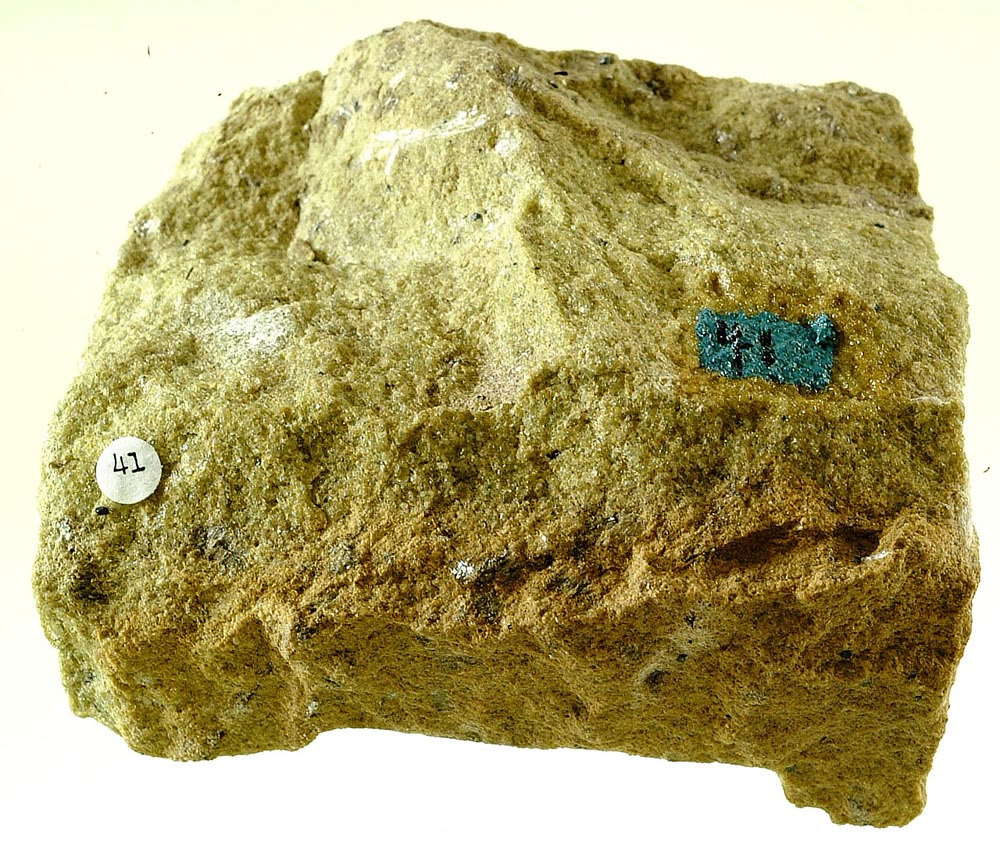
\includegraphics[width=\linewidth]{images/book4/b2-dunite.jpg}
\par\smallskip{\scriptsize 一块\omterm{def:b2:mantle-melting:peridotites}{纯橄岩}，几乎全由橄榄石组成，含细小的黑色
铬铁矿颗粒；样品宽 \qty{8.5}{cm}（照片：Mike Davis，CC0）。}
\end{minipage}
\end{inthefield}
% ledger: casetta23:kimberlite, tulane:ocean-basins (Book 2), bgs:ultramafic

\section{练习}

\begin{exercise}[$\star$]\label{exo:b2:mantle-melting:1}
根据橄榄石、斜方辉石与单斜辉石的百分含量命名每种岩石
（百分比）：(a) 93, 5, 2；(b) 75, 25, 0；(c) 60, 27, 13；(d) 30, 45, 25。(e) 将模型上地幔
（57, 28, 13 及 \qty{2}{\percent} 尖晶石）的三种硅酸盐重新归一化至 \qty{100}{\percent} 后，
给出其名称。
\end{exercise}
% ledger: bgs:ultramafic, liang21:dmm-mode

\begin{exercise}[$\star$]\label{exo:b2:mantle-melting:2}
在透辉石–钙长石图上，含 \qty{60}{\percent} 钙长石的液体
冷却。(a) 它在何温度开始结晶，
析出何种矿物？(b) 第二种矿物在何温度出现，
此时液相的成分如何？(c) 将含 \qty{80}{\percent} 透辉石与
\qty{20}{\percent} 钙长石的岩石加热时，第一个液相的成分为何，
在何温度出现？
\end{exercise}
% ledger: bowen15:di-an

\begin{exercise}[$\star$]\label{exo:b2:mantle-melting:3}
(a) 计算绝热梯度 $\alpha T/(\rho c_p)$，单位为开尔文每吉帕。
取 $T_p = \qty{1350}{\celsius}$，$\alpha = \qty{4.0e-5}{K^{-1}}$，$\rho =
\qty{3300}{kg/m^3}$，$c_p = \qty{1000}{J/(kg.K)}$。(b) 需多少千米厚的
地幔才能产生一吉帕的压强（$g = \qty{9.81}{m/s^2}$）？将梯度换算为开尔文
每千米，并与地表附近典型的地温梯度比较，
后者约为 \qty{30}{K/km}。
\end{exercise}
% ledger: katz03:thermo, earle:settings (Book 2)

\begin{exercise}[$\star$]\label{exo:b2:mantle-melting:4}
(a) 计算\omterm{def:b2:mantle-melting:peridotites}{橄榄岩}在 0、1、2 和 \qty{3}{GPa} 时的干固相线。(b) 在
\qty{2}{GPa} 附近，每吉帕升高多少度？(c) 用一句话说明
为何 \qty{3}{GPa} 下 \qty{1400}{\celsius} 的地幔呈固态，而
同一地幔在不与外界交换热量的情况下降压至 \qty{2}{GPa} 时\omterm{def:b2:mantle-melting:melting}{部分熔融}。
\end{exercise}
% ledger: katz03:solidus

\begin{exercise}[$\star\star$]\label{exo:b2:mantle-melting:5}
含 \qty{70}{\percent} 透辉石与 \qty{30}{\percent} 钙长石的液体冷却。
(a) 估算其液相线温度，方法是在钙长石含量为
\qty{20}{\percent}（\qty{1350}{\celsius}）与 \qty{40}{\percent}
（\qty{1277.5}{\celsius}）时的液相线之间插值。(b) 哪种矿物先结晶？(c) 液体到达低共熔点时，
体系中已结晶部分的质量分数为多少？
(d) 最终岩石中透辉石与钙长石的比例各为多少？
\end{exercise}
% ledger: bowen15:di-an

\begin{exercise}[$\star\star$]\label{exo:b2:mantle-melting:6}
(a) 计算 \ce{SiO2} 在镁橄榄石 \ce{Mg2SiO4} 与
顽火辉石 \ce{MgSiO3} 中的质量百分数（$M_{\ce{MgO}} = \qty{40.30}{g/mol}$，$M_{\ce{SiO2}} =
\qty{60.08}{g/mol}$）。(b) 鲍文与安德森发现\omterm{def:b2:mantle-melting:peritectic}{转熔点}液相为
\qty{97.5}{\percent} \ce{MgSiO3} 与 \qty{2.5}{\percent} \ce{SiO2}，其二氧化硅含量为多少？
(c) 用杠杆规则计算顽火辉石在\omterm{def:b2:mantle-melting:peritectic}{转熔点}熔化时生成的镁橄榄石质量分数，
并与他们给出的
\qty{5.5}{\percent} 比较。(d) 这对\omterm{def:b2:mantle-melting:peridotites}{橄榄岩}熔体的二氧化硅含量
与其斜方辉石相比有何启示？
\end{exercise}
% ledger: bowen14:mgo-sio2

\begin{exercise}[$\star\star$]\label{exo:b2:mantle-melting:7}
取绝热线 $T = T_p + 20P$ 与正文中的干固相线，计算熔化开始时的
压强与深度（每吉帕 $\qty{30.9}{km}$），分别对应
(a) $T_p = \qty{1300}{\celsius}$ 与 (b) $T_p = \qty{1450}{\celsius}$。
(c) 在 $T_p = \qty{1300}{\celsius}$ 附近，每升高 \qty{10}{\celsius}，
熔化起始深度增加多少千米？利用\cref{prop:b2:mantle-melting:onset}。
\end{exercise}
% ledger: katz03:solidus

\begin{exercise}[$\star\star$]\label{exo:b2:mantle-melting:8}
在 \qty{2.0}{GPa} 下，设\omterm{def:b2:mantle-melting:fraction}{熔体分数}自干固相线线性升至
\omterm{def:b2:mantle-melting:peridotites}{二辉橄榄岩}液相线 $T_{\mathrm l} = 1475.0 + 80.0P - 3.2P^2$。对于 $F = 0.10$：
(a) 计算正在熔融的岩石的温度；(b) 计算 $(\partial
T/\partial P)_F$ 与 $(\partial T/\partial F)_P$；(c) 计算产率，取
$c_p = \qty{1000}{J/(kg.K)}$，$\alpha/\rho = \qty{1.21e-8}{m^3/(kg.K)}$ 及
$\Delta S = \qty{300}{J/(kg.K)}$。(d) 若不计潜热，产率为多少？
\end{exercise}
% ledger: katz03:solidus, katz03:melting, katz03:thermo

\begin{exercise}[$\star\star$]\label{exo:b2:mantle-melting:9}
(a) 溶于熔体中的 1、5 和 \qty{13}{\percent} 的水分别使
固相线降低多少？(b) 在 \qty{1}{GPa} 下，水饱和固相线为多少？(c) 某地幔
含水质量分数为 \qty{125}{ppm}，且水在矿物与熔体间的分配系数
为 0.01。在最初开始熔融时，熔体中的含水量为 $X =
X_{\text{总体}}/D$：计算该值，以及由此引起的固相线降低量。
\end{exercise}
% ledger: katz03:water

\begin{exercise}[$\star\star\star$]\label{exo:b2:mantle-melting:10}
(a) 在\cref{prop:b2:mantle-melting:triangle}中，验证每年进入
三角形底边的地幔量等于从两侧流出的地幔量。为何
两侧必须呈 \ang{45}，对于以速率 $U$ 上升并以 $U$ 流出的地幔？
(b) 证明：在每吉帕产率 $\Pi$ 恒定时，$h_c = \Pi\,\rho
g\,z_0^2/2$（其中 $P_0 = \rho g z_0$），因此地壳厚度正比于
熔化起始深度的平方。(c) 某洋脊以 \qty{50}{mm/\text{年}} 的全扩张速率
生成 \qty{7.1}{km} 厚的地壳：每年每千米洋脊形成多少体积的地壳，
又熔融多少体积的地幔（若平均\omterm{def:b2:mantle-melting:fraction}{熔体分数}为
\qty{12}{\percent}）？
\end{exercise}

\begin{exercise}[$\star\star\star$]\label{exo:b2:mantle-melting:11}
在示意图所示的三元体系中，液体 $X$ 含
\qty{60}{\percent} A、\qty{20}{\percent} B 和 \qty{20}{\percent} C；二元
低共熔点 $e_{AB}$ 位于 A 40、B 60（百分数），\omterm{def:b2:mantle-melting:ternary}{三元共晶点} E 位于
A 25、B 30、C 45。(a) 写出纯 A 的质量分数 $t$ 结晶后液体的成分，
并证明 B 与 C 之比保持为 1。(b) 从
$e_{AB}$ 到 E 的\omterm{def:b2:mantle-melting:ternary}{共结线}为点集 $e_{AB} + s(E - e_{AB})$：求
液体与之相交的位置，以及此时已结晶的 A 的比例。(c) 当
液体到达 E 时，体系中仍为液相的比例为多少？（在到达 E 之前，C 不进入
任何晶体。）(d) 到那时，已结晶的 A 与 B 各为多少？
\end{exercise}

\begin{exercise}[$\star\star\star$]\label{exo:b2:mantle-melting:12}
饱和熔体的含水量为 $X_{\mathrm{sat}} = 12P^{0.6} + P$
（百分数，$P$ 以吉帕计）。(a) 计算其在 1 和 \qty{2}{GPa} 时的值，由此得到的固相线
降低量，以及两压强下的水饱和固相线。(b) 为何
在 1 至 \qty{2}{GPa} 之间，饱和固相线几乎不变，而干固相线
升高超过 \qty{100}{\celsius}？(c) 在 \qty{2}{GPa} 与
\qty{1100}{\celsius} 的地幔楔中，熔体须含多少水，岩石才会熔融？
\end{exercise}
% ledger: katz03:water, katz03:solidus

\section{问题：洋脊之下}

\begin{problem}[{周末问题——从地幔绝热线到洋壳厚度，
再回到地幔温度}]
\label{pb:b2:mantle-melting:1}
地幔沿绝热线在洋脊之下上升并发生熔融。已知数据：热膨胀系数
$\alpha = \qty{4.0e-5}{K^{-1}}$；密度 $\rho = \qty{3300}{kg/m^3}$；
比热容 $c_p = \qty{1000}{J/(kg.K)}$；熔化熵 $\Delta S =
\qty{300}{J/(kg.K)}$；$g = \qty{9.81}{m/s^2}$；干固相线 $T_{\mathrm s} =
1085.7 + 132.9P - 5.1P^2$，\omterm{def:b2:mantle-melting:peridotites}{二辉橄榄岩}液相线 $T_{\mathrm l} = 1475.0 +
80.0P - 3.2P^2$（\unit{\celsius}，$P$ 以 \unit{GPa} 计）；拟合熔融模型的
平均产率 $\Pi = \qty{9}{\percent}$ 每吉帕；近地表的单斜辉石
反应系数为 0.50；观测到的地壳厚度在正常洋脊处为 \qty[uncertainty-mode=separate]{7.1 \pm 0.8}{km}，
冰岛地幔柱核心上方为 \qty{20}{km}。假设地幔
与地壳密度相同。

\noindent\textbf{第一部分——熔融始于何处。}
\begin{enumerate}
\item 将 $T_p = \qty{1350}{\celsius}$ 换算为开尔文。
\item 计算绝热梯度 $\alpha T_p/(\rho c_p)$，单位为开尔文每
吉帕，并将结果取整到最近的十位。
\item 一吉帕对应多少千米的地幔？以开尔文每
千米表示该梯度。
\item 取绝热线 $T = 1350 + 20P$，写出起始压力
$P_0$ 所满足的二次方程并求解。
\item 给出熔融开始处的深度和温度。
\item 验证在 $P_0$ 处的固相线给出相同的温度。
\end{enumerate}

\noindent\textbf{第二部分——熔体的量。}
\begin{enumerate}[resume]
\item 在 \qty{1.5}{GPa} 处，计算固相线、\omterm{def:b2:mantle-melting:peridotites}{二辉橄榄岩}液相线
及二者之差。
\item 设\omterm{def:b2:mantle-melting:fraction}{熔体分数}在二者之间线性增加，求岩石在
$F = 0.10$ 处的温度，分别以摄氏度和开尔文表示。
\item 计算该点处的 $(\partial T/\partial P)_F$ 和 $(\partial T/\partial F)_P$。
\item 计算\cref{prop:b2:mantle-melting:productivity}中的
产率，以每吉帕的百分数表示。
\item 拟合模型给出的平均产率为 $\Pi = \qty{9}{\percent}$ 每吉帕。
为何它更低？利用 $\Pi$，
求地表所达到的\omterm{def:b2:mantle-melting:fraction}{熔体分数} $F_{\max}$？
\item 模型地幔含 \qty{13}{\percent} 的单斜辉石。在何种
\omterm{def:b2:mantle-melting:fraction}{熔体分数}下，其在近地表处被耗尽？轴下方的残余体是
\omterm{def:b2:mantle-melting:peridotites}{二辉橄榄岩}还是\omterm{def:b2:mantle-melting:peridotites}{方辉橄榄岩}？
\end{enumerate}

\noindent\textbf{第三部分——地壳。}
\begin{enumerate}[resume]
\item 取 $H = z_0$，利用\cref{prop:b2:mantle-melting:triangle}
计算地壳厚度。
\item 汇集熔体的平均\omterm{def:b2:mantle-melting:fraction}{熔体分数}是多少？
\item 与观测厚度进行比较。
\item 图中完整模型给出 \qty{9.0}{km}。为何它比
你的估算值更薄？
\item 证明 $h_c = k P_0^2$，并计算 $k$，
单位为千米每平方吉帕。
\end{enumerate}

\noindent\textbf{第四部分——地幔的温度。}
\begin{enumerate}[resume]
\item 计算使地壳厚度为 \qty{7.1}{km} 的起始压力 $P_0$。
\item 给出对应的起始深度。
\item 取绝热线 $T = T_p + 20P$，计算使起始
发生在该压力处的位温。
\item 对 6.3 和 \qty{7.9}{km} 重做计算：地壳
厚度的散布允许 $T_p$ 处于怎样的范围？
\item 冰岛地幔柱核心上方的地壳厚度为 \qty{20}{km}。
计算该处的位温，及其相对第~20~题所求位温的超出量。
\item 洋岛熔岩表明，地幔柱比周围地幔热
200 至 \qty{300}{\celsius}。试说明为何地壳给出的超出量较小。
\item 在正常洋脊附近，地幔高 \qty{10}{\celsius} 时，
地壳增厚了百分之几？
\item 极慢速洋脊形成较薄的地壳，请利用三角图解释其原因。
\item 由正常洋脊之下地壳的厚度，给出
该处地幔的位温，这是本题的关键数值，并将其与
矿物物理给出的 \qty{1350}{\celsius} 以及由熔岩得出的 1280 至
\qty{1400}{\celsius} 范围进行比较。
\end{enumerate}
\end{problem}
% ledger: katz03:solidus, katz03:melting, katz03:thermo, white:crust (Book 3), herzberg:tp (Book 3), katsura:adiabat (Book 3)
